\section*{3. Background and Related Concepts}

\begin{figure*}[t]
  \centering
  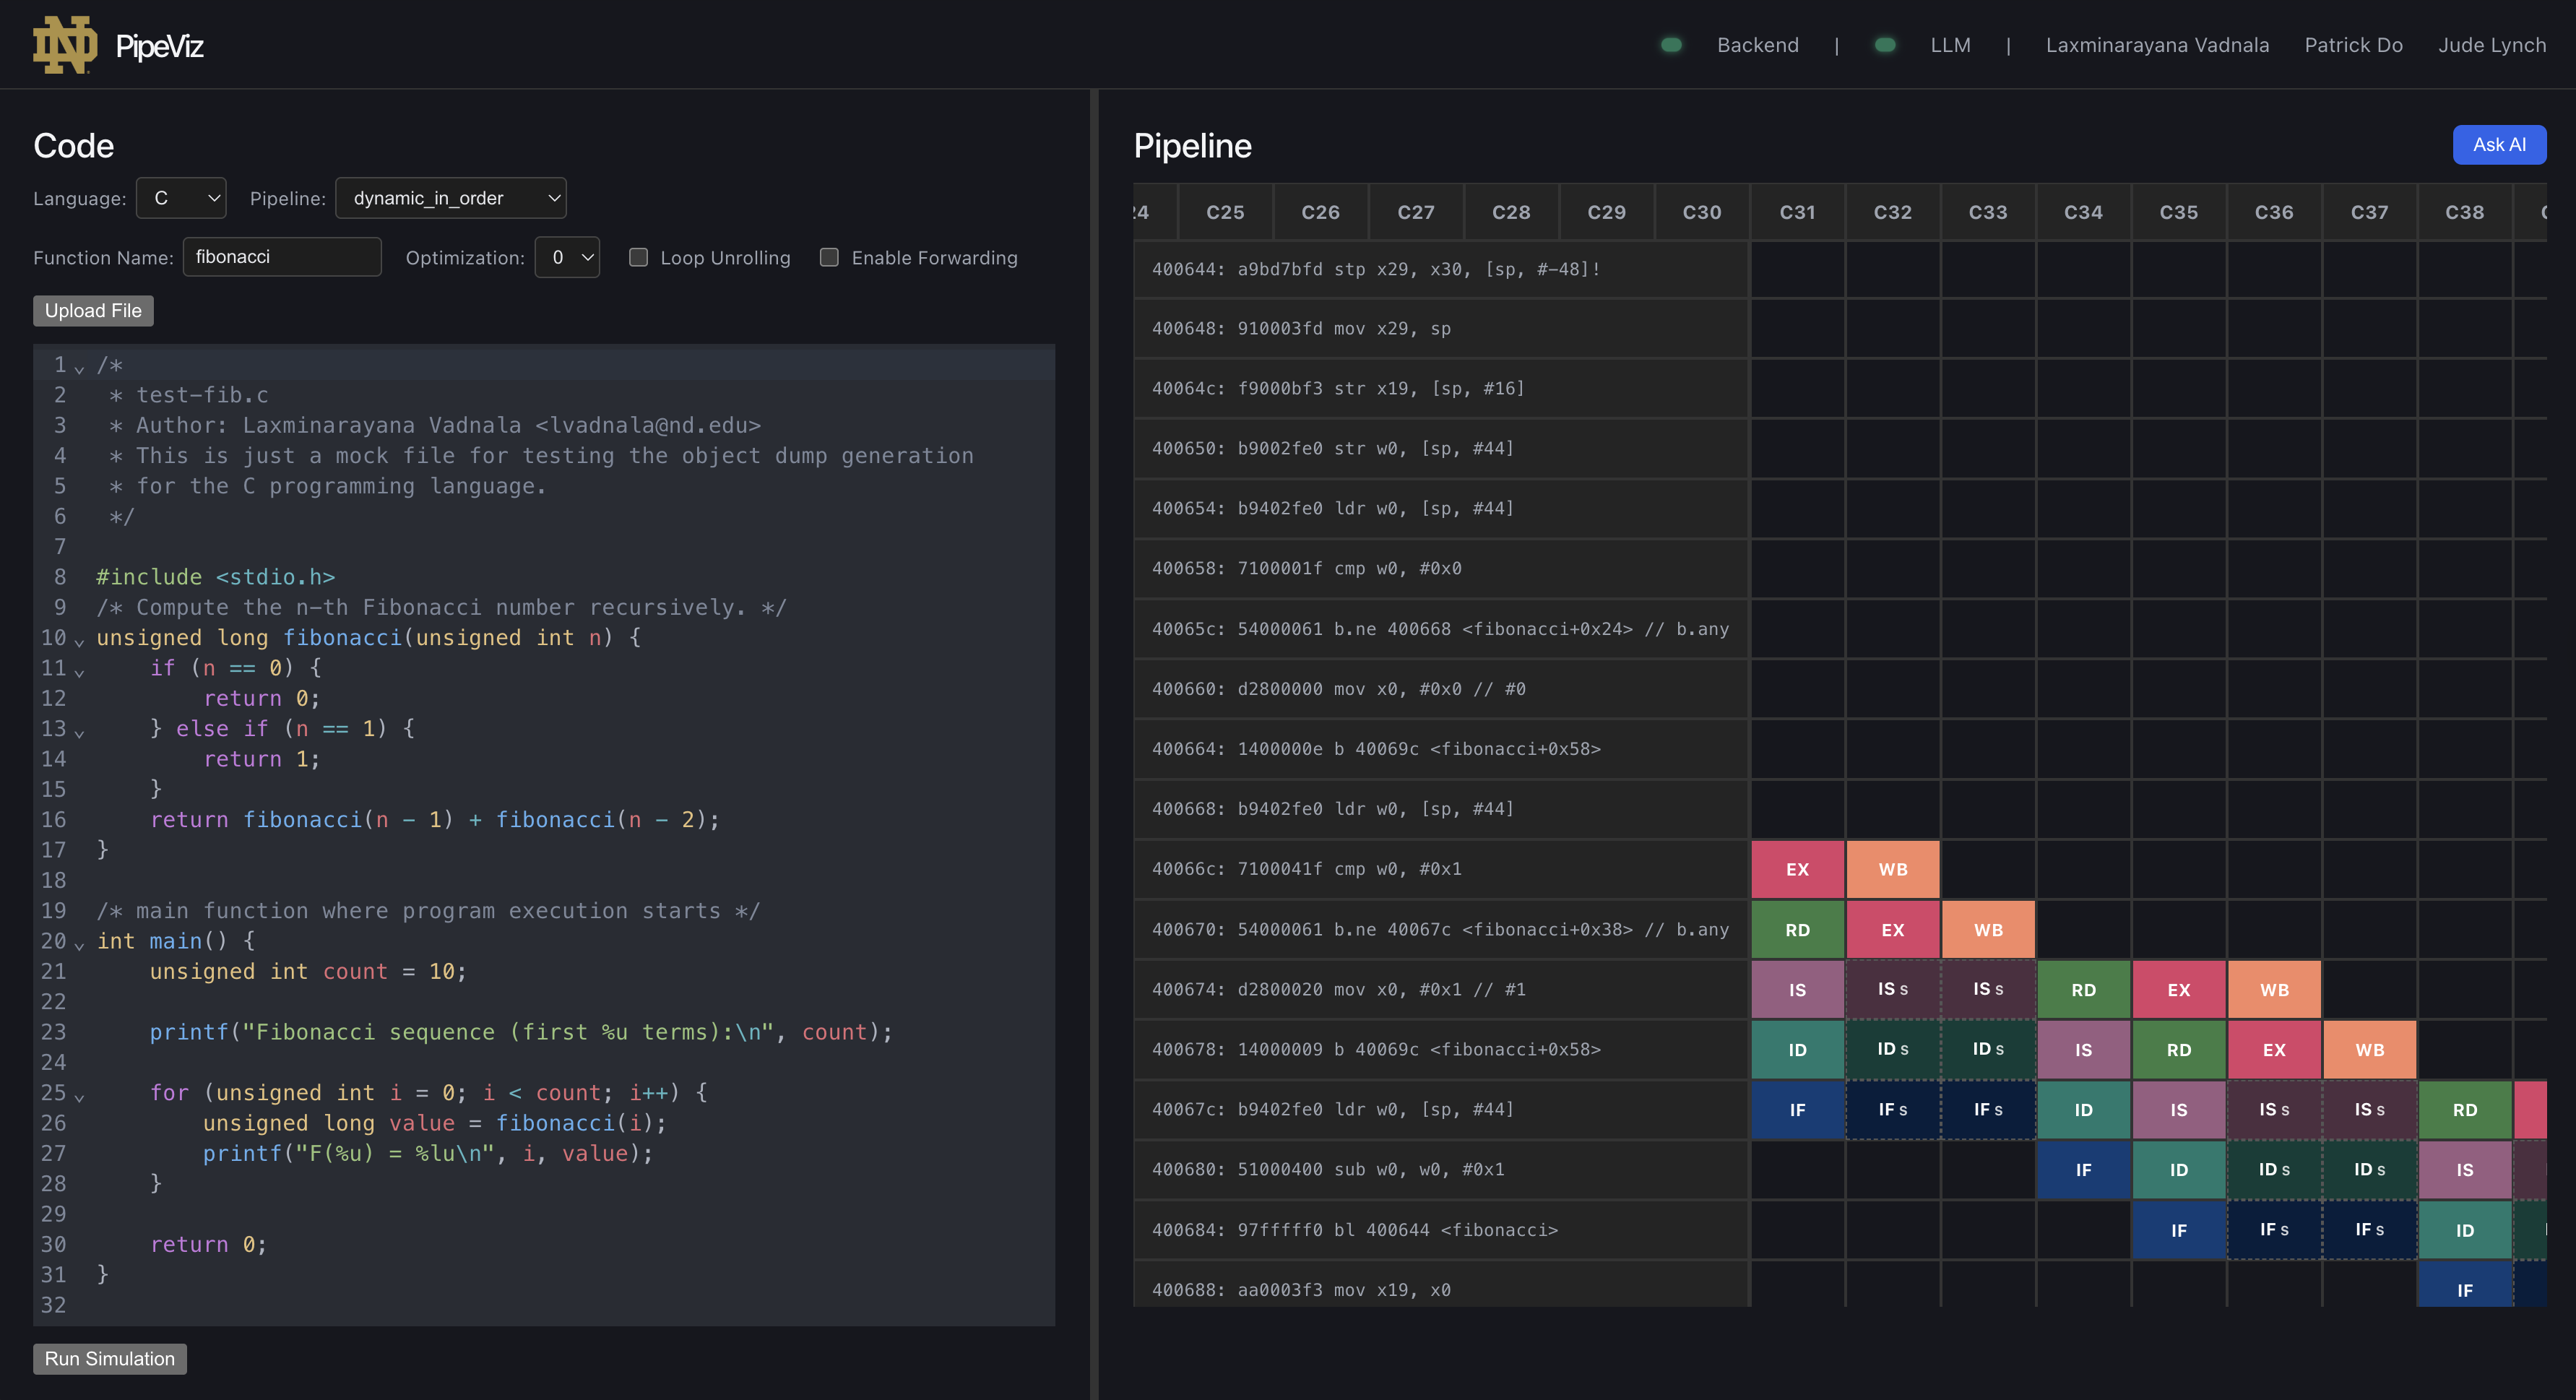
\includegraphics[width=\textwidth]{fig/pipeviz_interface.png}
  \vspace{-0.25in}
  \caption{The PipeViz user interface. The left panel provides a code editor with controls for language, pipeline model, target function, optimization level, loop unrolling, and data forwarding. The right panel displays the cycle-by-cycle pipeline execution table, where each row corresponds to an AArch64 instruction and each column represents a clock cycle. Stage labels are color-coded to indicate each instruction's progression through the pipeline.} 
  \label{fig:interface}
\end{figure*}

\subsection*{3.1 Pipeline Execution}
In a classic in-order pipeline, instructions progress through stages (fetch, decode, execute, memory, write back). Each cycle, ideally, one instruction advances to the next stage. Real execution deviates from this ideal due to dependencies and resource conflicts.


\subsection*{3.2 Data Hazards}
PipeViz detects three major data hazards: \\
(1) \textbf{RAW (Read After Write)}: An instruction reads a register before a previous instruction writes it. \\ 
(2) \textbf{WAR (Write After Read)}: An instruction writes a register before a previous instruction has read it.  \\
(3) \textbf{WAW (Write After Write)}: Two instructions write the same register in the wrong order.  \\


These hazards cause stalls when the pipeline must wait for a value to become available.

\subsection*{3.3 Structural Hazards}
Structural hazards occur when two or more instructions require the same hardware resource in the same cycle (e.g., memory access). This creates contention and stalls.

\subsection*{3.4 Compiler and Code Optimizations}
Compiler optimizations such as instruction scheduling, strength reduction, and loop unrolling often reduce hazards by increasing independence between instructions and improving utilization of pipeline stages. PipeViz leverages an LLM to suggest similar optimizations when a user observes frequent stalls.

